% \input{"IAB/latex/TeX-Folienformat.tex"}
\input{"/Users/jonathanlatner/Google Drive/My Drive/IAB/latex/TeX-Folienformat.tex"}

\documentclass[t,8pt,utfx8]{beamer}
\usepackage{booktabs}
\usepackage{setspace}
\usepackage{parskip}
\usepackage{graphicx}
\usepackage{subcaption}
\setbeamertemplate{caption}[numbered]
\newcommand{\sprache}{\englisch}
\renewcommand{\thesubsection}{\alph{subsection})}
\usepackage[cal=pxtx, scr=dutchcal]{mathalpha}
\usepackage{forest}



\definecolor{codegreen}{rgb}{0,0.6,0}
\definecolor{codegray}{rgb}{0.5,0.5,0.5}
\definecolor{codepurple}{rgb}{0.58,0,0.82}
\definecolor{backcolour}{rgb}{0.95,0.95,0.92}


\usepackage{listings}

% Define style for R code
\lstset{
  language=R,
  basicstyle=\ttfamily\small,
  keywordstyle=\color{blue},
  stringstyle=\color{red},
  commentstyle=\color{green},
  showstringspaces=false,
  numbers=left,
  numberstyle=\tiny\color{gray},
  stepnumber=1,
  numbersep=5pt,
  breaklines=true,
  frame=single
}

\newcommand{\btVFill}{\vskip0pt plus 1filll}


\title{Buyer Beware: Understanding the trade-off between utility and risk in CART based models using simulation data}

\author{Jonathan Latner, PhD \newline Dr. Marcel Neunhoeffer \newline Prof. Dr. Jörg Drechsler}

\newcounter{noauthorlines}
\setcounter{noauthorlines}{2} % Wert für 2 Autoren über 2 Zeilen. Ggf. anpassen

% %%%%%%%%%%%%%%
% Ende Anpassung
% %%%%%%%%%%%%%%

% \input{"IAB/latex/TeX-Folienformatierung_CD_2019"}
\input{"/Users/jonathanlatner/Google Drive/My Drive/IAB/latex/TeX-Folienformatierung_CD_2019"}

% Modify the section in toc template to enumerate
\setbeamertemplate{section in toc}{%
    \inserttocsectionnumber.~\inserttocsection\par
}

% use for subsections
% \setbeamertemplate{subsection in toc}{}
\setbeamertemplate{subsection in toc}{%
    \setlength{\parskip}{1mm}
        \hskip2mm -- \hskip1mm\inserttocsubsection\par
}


\usepackage{colortbl}
\definecolor{lightgray}{gray}{0.9}

\usepackage{listings} %include R code
\lstdefinestyle{mystyle}{
    backgroundcolor=\color{backcolour},   
    commentstyle=\color{codegreen},
    keywordstyle=\color{magenta},
    numberstyle=\tiny\color{codegray},
    stringstyle=\color{codepurple},
    basicstyle=\ttfamily\tiny,
    breakatwhitespace=false,         
    breaklines=true,                 
    captionpos=b,                    
    keepspaces=true,                 
    numbers=left,                    
    numbersep=5pt,                  
    showspaces=false,                
    showstringspaces=false,
    showtabs=false,                 
    columns=fullflexible,
    frame=single,
    tabsize=2
}
\lstset{style=mystyle}


\begin{document}


\frame[plain]{\titlepage}

\begin{spacing}{1.25}

%%%%%%%%%%%%%%%%%%%%%%%%%%%%%%%%%%%%%%%%
%%%%%%%%%%%%%%%%%%%%%%%%%%%%%%%%%%%%%%%%
\section{The data}\label{sec:data}
%%%%%%%%%%%%%%%%%%%%%%%%%%%%%%%%%%%%%%%%
%%%%%%%%%%%%%%%%%%%%%%%%%%%%%%%%%%%%%%%%
\begin{frame}[c,plain]
\vskip-4mm
\begin{beamercolorbox}[wd=\boxwidth,ht=22.11mm]{transparent}%
    \vfill%
    \usebeamerfont{title}%
    \leftinsert%
    \MakeUppercase{Section \ref{sec:data}: Generate the original and synthetic data
} % <- Hier die Überschrift eintragen
\end{beamercolorbox}
\vskip-3mm
\pgfuseimage{rahmenlinie}
\begin{itemize}
    \item Borrowing from Reiter et al. (2014), we create a data set with $n=1000$ and 4 dichotomous, categorical variables. 
    \item The first 999 observations to be a random sample from a multinomial distribution for all combinations of $var1(0,1), var2(0,1), var3(0,1), var4(0,1)$ except the last one
    \item The last (1000$^{th}$) observation is ($var1=1,var2=1,var3=1,var4=1$). 
\end{itemize}

\end{frame}

\frame{\frametitle{Generate original data using a simulation}
\begin{minipage}{0.48\textwidth}
    \begin{figure}
        \centering
        \caption{Frequency}
        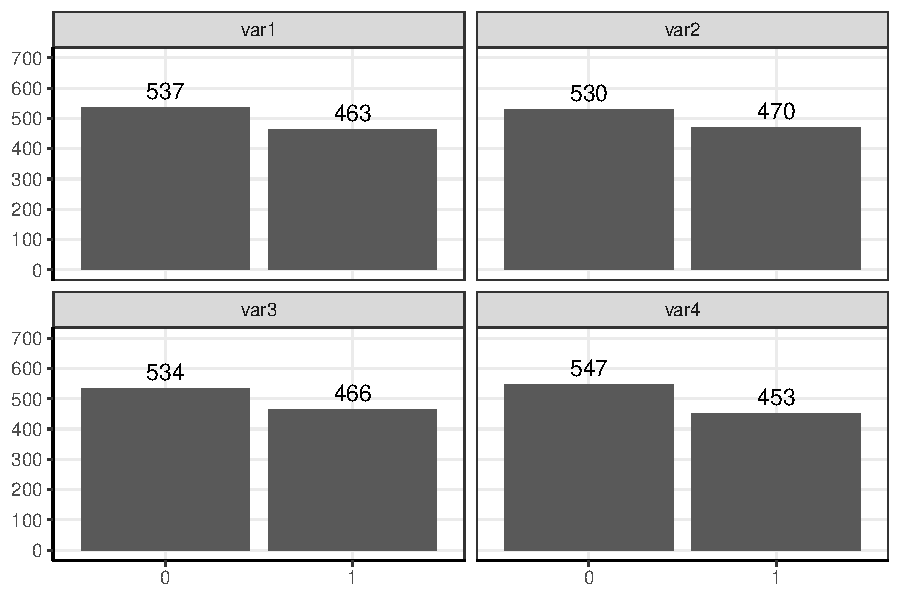
\includegraphics[width=\textwidth]{../../graphs/graph_cart_frequency.pdf}
    \end{figure}
\end{minipage}
\hfill
\begin{minipage}{0.48\textwidth}
    \begin{figure}
        \centering
        \caption{Histogram}
        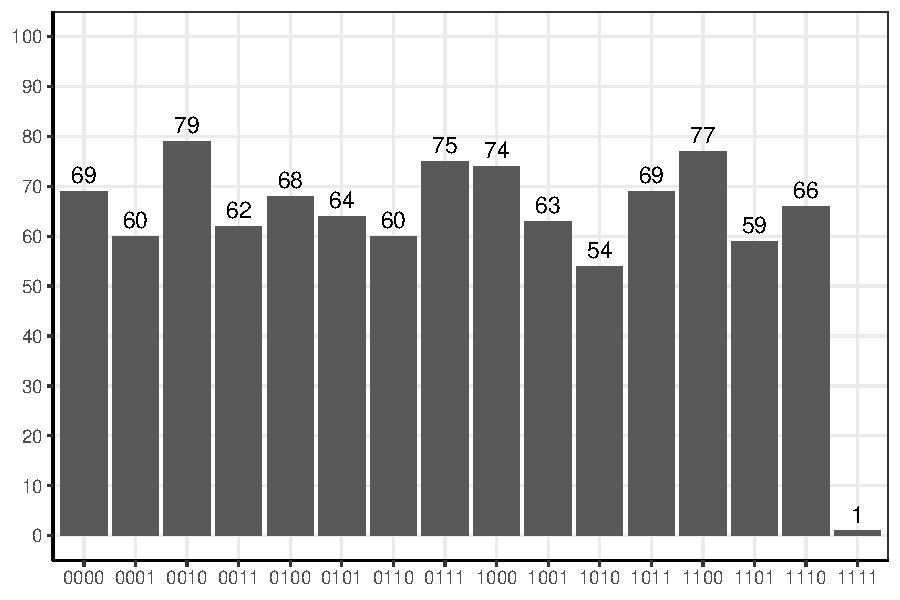
\includegraphics[width=\textwidth]{../../graphs/graph_cart_histogram.pdf}
    \end{figure}
\end{minipage}

}


\frame{\frametitle{Generate synthetic data with CART (synthpop)}

\begin{minipage}{0.48\textwidth}
    \begin{figure}
        \centering
        \caption{Frequency}
        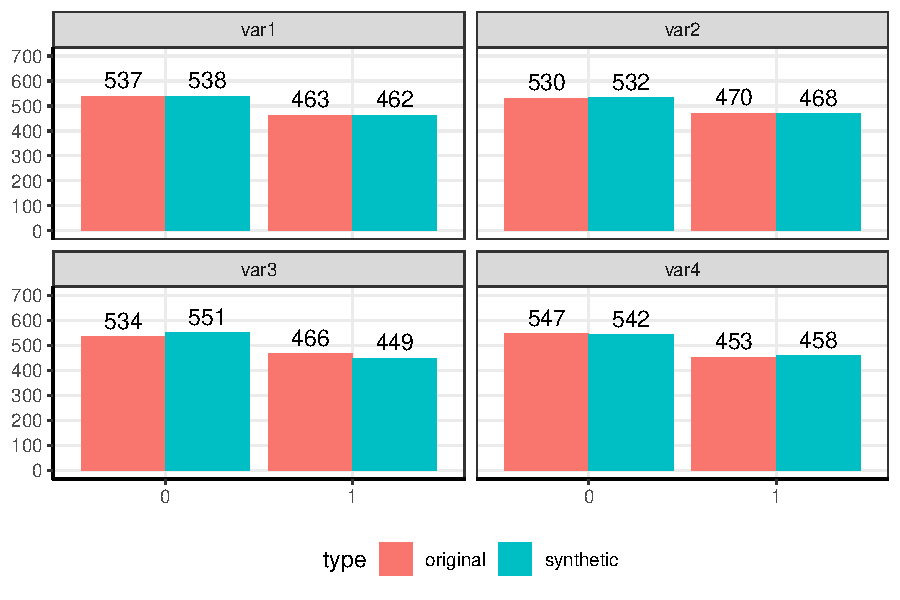
\includegraphics[width=\textwidth]{../../graphs/graph_cart_frequency_compare.pdf}
    \end{figure}
\end{minipage}
\hfill
\begin{minipage}{0.48\textwidth}
    \begin{figure}
        \centering
        \caption{Histogram}
        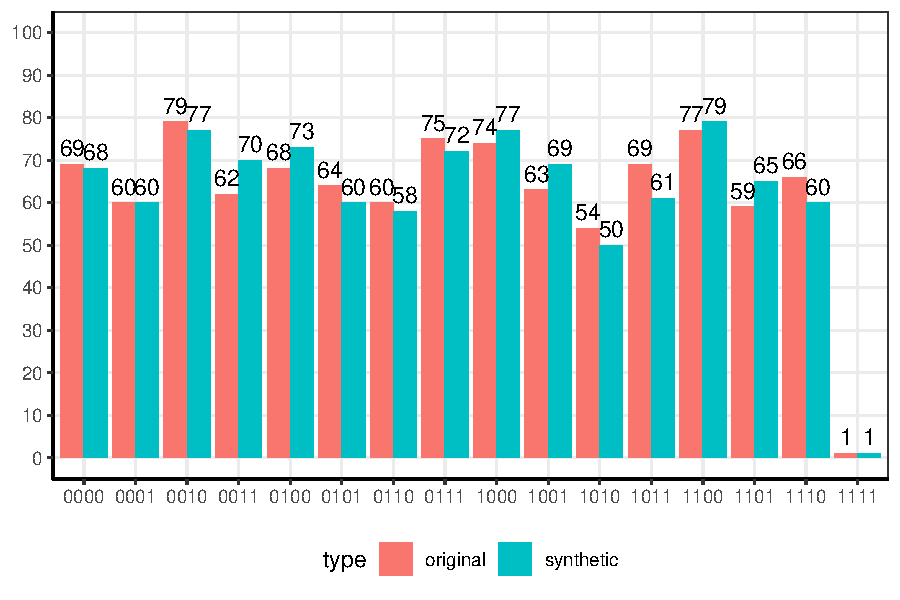
\includegraphics[width=\textwidth]{../../graphs/graph_cart_histogram_compare.pdf}
    \end{figure}
\end{minipage}

}


\frame{\frametitle{Compare histogram x 10 synthetic datasets}
\begin{figure}
    \caption{Multiple synthetic data sets does not reduce privacy risk}
    \resizebox{\textwidth}{!}{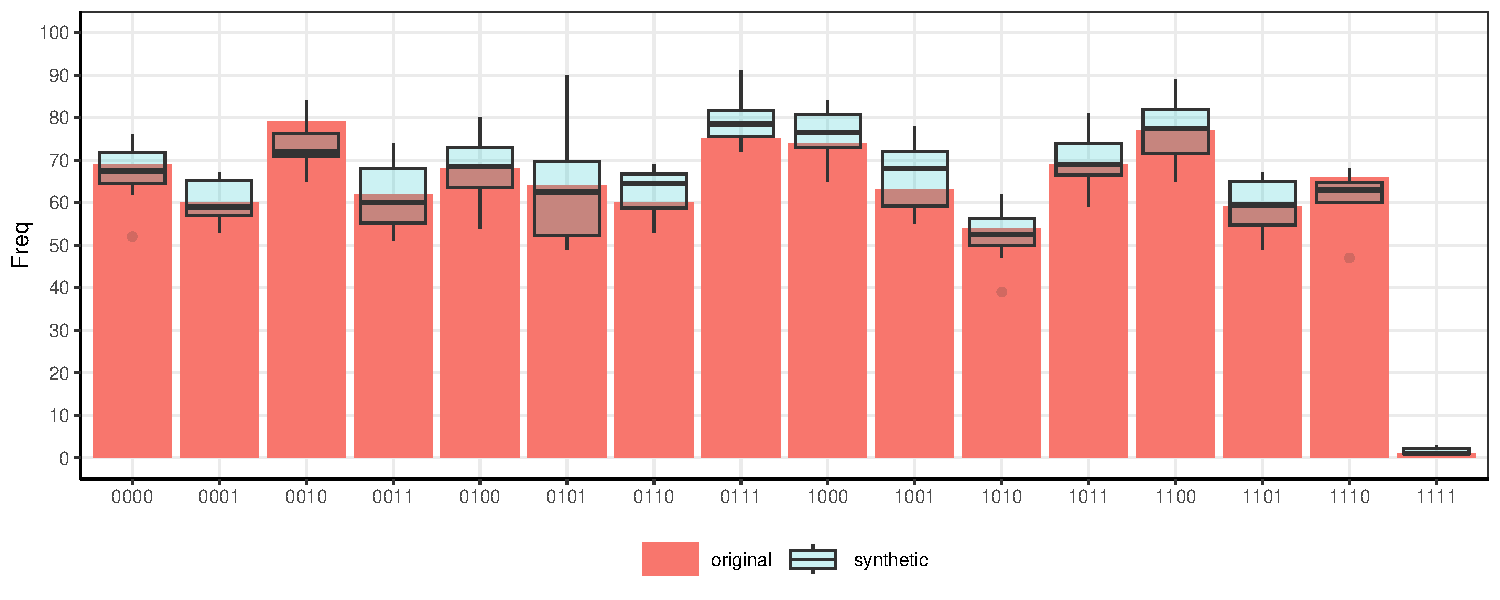
\includegraphics{../../graphs/graph_cart_histogram_compare_10.pdf}}
    \label{fig:graph_cart_histogram_compare_10}
\end{figure}
}

\frame{\frametitle{Summary}
\begin{itemize}
    \item The problem (in our data): Synthetic data from CART models are disclosive
    \item The reason: 
    \begin{itemize}
        \item A record can only be in the synthetic data if it is also in the original data (in this simulated data).   
        \item Or the opposite: if a record is not in the original data, then it can never be in the synthetic data.
    \end{itemize}  
    \item Next section: Can an attacker identify the disclosure?
\end{itemize}
}

%%%%%%%%%%%%%%%%%%%%%%%%%%%%%%%%%%%%%%%%
%%%%%%%%%%%%%%%%%%%%%%%%%%%%%%%%%%%%%%%%
\section{The attack}\label{sec:attack}
%%%%%%%%%%%%%%%%%%%%%%%%%%%%%%%%%%%%%%%%
%%%%%%%%%%%%%%%%%%%%%%%%%%%%%%%%%%%%%%%%
\begin{frame}[c,plain]
\vskip-4mm
\begin{beamercolorbox}[wd=\boxwidth,ht=22.11mm]{transparent}%
    \vfill%
    \usebeamerfont{title}%
    \leftinsert%
    \MakeUppercase{Section \ref{sec:attack}: The attack
} % <- Hier die Überschrift eintragen
\end{beamercolorbox}
\vskip-3mm
\pgfuseimage{rahmenlinie}

\end{frame}

\frame{\frametitle{Describing the attack}
\begin{itemize}
    \item We assume a `strong' attacker similar to the attack model in differential privacy (DP). 
    \item An attacker has the following knowledge
    \begin{itemize}
        \item Knows the SDG model type (i.e. sequential CART).
        \item Knowledge of all observations in the data except the last one.  
        \item The 16 possible combinations that the last one could be.
    \end{itemize}
    \item The attacker sees the synthetic data
    \item The attacker runs the same synthetic data model (SDG) for all of the 16 different possibilities.  
    \item Then they update their beliefs about what the last record could be
\end{itemize}
}


\frame{\frametitle{Illustrating the attack with CART (default parameters)}
\vskip -3mm
\begin{figure}
    \caption{Histogram of 16 worlds x 100 synthetic datasets}
    \vskip -4mm
    \resizebox{\textwidth}{!}{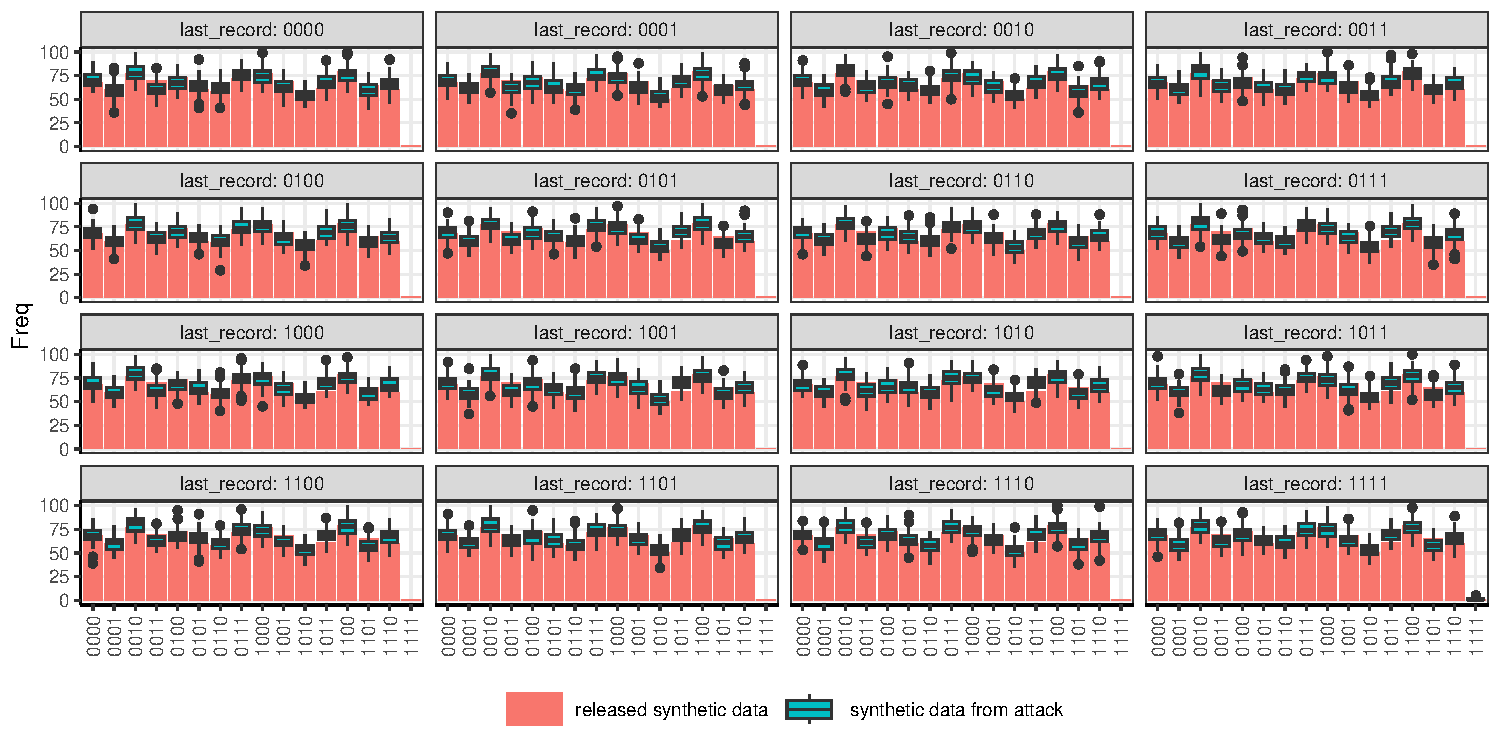
\includegraphics{../../graphs/graph_attacker_default.pdf}}
    \label{fig:graph_attacker_default}
\end{figure}
}


\frame{\frametitle{Summary}
\begin{itemize}
    \item In our attack with our assumptions, the attacker can easily identify the last record
    \item The reason (to repeat): 
    \begin{itemize}
        \item A record can only be in the synthetic data if it is also in the original data (in this simulated data).   
        \item Or the opposite: if a record is not in the original data, then it can never be in the synthetic data.
    \end{itemize}  
    \item Next section: Can we measure this disclosure?
\end{itemize}

}


%%%%%%%%%%%%%%%%%%%%%%%%%%%%%%%%%%%%%%%%
%%%%%%%%%%%%%%%%%%%%%%%%%%%%%%%%%%%%%%%%
\section{Measuring privacy}\label{sec:privacy}
%%%%%%%%%%%%%%%%%%%%%%%%%%%%%%%%%%%%%%%%
%%%%%%%%%%%%%%%%%%%%%%%%%%%%%%%%%%%%%%%%
\begin{frame}[c,plain]
\vskip-4mm
\begin{beamercolorbox}[wd=\boxwidth,ht=22.11mm]{transparent}%
    \vfill%
    \usebeamerfont{title}%
    \leftinsert%
    \MakeUppercase{Section \ref{sec:privacy}: Measuring privacy
} % <- Hier die Überschrift eintragen
\end{beamercolorbox}
\vskip-3mm
\pgfuseimage{rahmenlinie}

The literature on privacy measures for synthetic data is well-developed (Wagner and Eckhoff, 2018).  

Common privacy measures - Synthpop (Raab et al., 2024)

\begin{itemize}
    \item Identity disclosure (\%): the ability to identify individuals in the data from a set of known characteristics or `keys' ($q$).  
    \item Attribute disclosure (\%): the ability to find out from the keys something, not previously known or `target' ($t$)
\end{itemize}

\end{frame}

\frame{\frametitle{Identity disclosure}

$repU$ (replicated uniques) are unique records in the original data that are also unique in synthetic data and is the measure of identity risk.  Formally, $repU$ is defined by equation \ref{eq:repU}:

\begin{equation}
repU = 100 \sum (s_{.q}|d_{.q} = 1 \land s_{.q} = 1 )/N_{d}
\label{eq:repU}
\end{equation}

where $d_{.q}$ is the count of records in the original data with the keys corresponding to a given value of $q$ and $s_{.q}$ is the equivalent count for the synthetic data.  

In a given value of $q$, $s_{.q}|d_{.q} = 1$ is a unique record in the original data conditional on also existing in the synthetic data.  

AND

$s_{.q} = 1$ is the unique record in the synthetic data.  

This is summed over unique values of $q$ and divided by the total number of records in the data ($N_{d}$) and multiplied by 100 to transform the count into a percentage.

}

\frame{\frametitle{Attribute disclosure}

$DiSCO$ (Disclosive in Synthetic Correct in Original) is the subset of records in the original data for which the keys ($q$) in the synthetic data is disclosive. $q$ is disclosive if all records in the synthetic data with the same $q$ have a constant target ($t$), i.e. no variation in $t$, as defined by the following equation \ref{eq:DiSCO}:

\begin{equation}
DiSCO = 100 \sum^{q} \sum^{t} (d_{tq} | ps_{tq} = 1) / N_{d}
\label{eq:DiSCO}
\end{equation}

where $d_{tq} | s_{tq} = 1$ indicates whether the synthetic data matches the original data for the combination of $t$ and $q$ given the condition that the synthetic data for the combination of $t$ and $q$ is disclosive (i.e., target $t$ is uniquely determined by the keys $q$).  

This is summed over unique values of $t$ and unique values of $q$ and divided by the total number of records in the data ($N_{d}$) and multiplied by 100 to transform the count into a percentage.
}


\begin{frame}[fragile]
\frametitle{Comparing disclosure risk measures}

\begin{minipage}[t]{0.48\textwidth}
    \begin{table}[]
        \centering
        \caption{x 1 synthetic data set (seed = 1237)}
        % latex table generated in R 4.4.0 by xtable 1.8-4 package
% Tue Jan 14 12:47:47 2025
\begin{tabular}{lrr}
  \toprule
data & identity & attribute \\ 
  \midrule
Original & 0.00 & 0.00 \\ 
  Synthetic & 0.00 & 0.00 \\ 
   \bottomrule
\end{tabular}

        \label{table:disclosure_risk_1}
    \end{table}
\end{minipage}%
\hfill%
\begin{minipage}[t]{0.48\textwidth}
    \begin{table}[]
        \centering
        \caption{x 10 synthetic data sets}
        % latex table generated in R 4.4.0 by xtable 1.8-4 package
% Tue Jan 14 12:47:47 2025
\begin{tabular}{lrr}
  \toprule
data & identity & attribute \\ 
  \midrule
Original & 0.00 & 0.00 \\ 
  Synthetic & 0.00 & 1.32 \\ 
   \bottomrule
\end{tabular}

        \label{table:disclosure_risk_10}
    \end{table}
\end{minipage}
\end{frame}


\begin{frame}[fragile]
\frametitle{Underlying information}
\vskip -3mm

\begin{minipage}[t]{0.48\textwidth}
    \begin{table}[]
        \centering
        \caption{Frequency statistics}
        \rowcolors{1}{white}{lightgray}
        \resizebox{\textwidth}{!}{% latex table generated in R 4.4.0 by xtable 1.8-4 package
% Mon Dec 16 16:27:40 2024
\begin{tabular}{lrrrrrrrrrrr}
  \toprule
   & \multicolumn{1}{l}{Original} & \multicolumn{10}{c}{Synthetic Data} \\ \cmidrule(lr){3-12}
 Combine & 0 & 1 & 2 & 3 & 4 & 5 & 6 & 7 & 8 & 9 & 10 \\ 
 \midrule
0000 & 69 & 68 & 66 & 71 & 73 & 76 & 62 & 72 & 52 & 64 & 67 \\ 
  0001 & 60 & 60 & 53 & 57 & 56 & 58 & 60 & 67 & 67 & 57 & 67 \\ 
  0010 & 79 & 77 & 71 & 73 & 71 & 71 & 84 & 65 & 70 & 77 & 74 \\ 
  0011 & 62 & 70 & 51 & 56 & 68 & 63 & 55 & 74 & 57 & 68 & 52 \\ 
  0100 & 68 & 73 & 63 & 80 & 54 & 61 & 79 & 65 & 73 & 66 & 71 \\ 
  0101 & 64 & 60 & 77 & 49 & 66 & 52 & 90 & 52 & 53 & 65 & 71 \\ 
  0110 & 60 & 58 & 68 & 66 & 61 & 69 & 56 & 67 & 65 & 64 & 53 \\ 
  0111 & 75 & 72 & 91 & 86 & 81 & 80 & 77 & 82 & 77 & 75 & 72 \\ 
  1000 & 74 & 77 & 84 & 80 & 73 & 70 & 81 & 82 & 65 & 76 & 73 \\ 
  1001 & 63 & 69 & 66 & 57 & 68 & 73 & 56 & 68 & 75 & 78 & 55 \\ 
  1010 & 54 & 50 & 54 & 57 & 51 & 47 & 50 & 39 & 62 & 58 & 54 \\ 
  1011 & 69 & 61 & 59 & 77 & 71 & 66 & 69 & 75 & 69 & 68 & 81 \\ 
  1100 & 77 & 79 & 77 & 76 & 83 & 78 & 66 & 65 & 88 & 70 & 89 \\ 
  1101 & 59 & 65 & 52 & 54 & 57 & 66 & 67 & 59 & 65 & 49 & 60 \\ 
  1110 & 66 & 60 & 68 & 60 & 64 & 68 & 47 & 65 & 62 & 64 & 60 \\ 
  1111 & 1 & 1 & 0 & 1 & 3 & 2 & 1 & 3 & 0 & 1 & 1 \\ 
   \bottomrule
\end{tabular}
}
        % % latex table generated in R 4.4.0 by xtable 1.8-4 package
% Mon Dec 16 16:27:40 2024
\begin{tabular}{lrrrrrrrrrrr}
  \toprule
   & \multicolumn{1}{l}{Original} & \multicolumn{10}{c}{Synthetic Data} \\ \cmidrule(lr){3-12}
 Combine & 0 & 1 & 2 & 3 & 4 & 5 & 6 & 7 & 8 & 9 & 10 \\ 
 \midrule
0000 & 69 & 68 & 66 & 71 & 73 & 76 & 62 & 72 & 52 & 64 & 67 \\ 
  0001 & 60 & 60 & 53 & 57 & 56 & 58 & 60 & 67 & 67 & 57 & 67 \\ 
  0010 & 79 & 77 & 71 & 73 & 71 & 71 & 84 & 65 & 70 & 77 & 74 \\ 
  0011 & 62 & 70 & 51 & 56 & 68 & 63 & 55 & 74 & 57 & 68 & 52 \\ 
  0100 & 68 & 73 & 63 & 80 & 54 & 61 & 79 & 65 & 73 & 66 & 71 \\ 
  0101 & 64 & 60 & 77 & 49 & 66 & 52 & 90 & 52 & 53 & 65 & 71 \\ 
  0110 & 60 & 58 & 68 & 66 & 61 & 69 & 56 & 67 & 65 & 64 & 53 \\ 
  0111 & 75 & 72 & 91 & 86 & 81 & 80 & 77 & 82 & 77 & 75 & 72 \\ 
  1000 & 74 & 77 & 84 & 80 & 73 & 70 & 81 & 82 & 65 & 76 & 73 \\ 
  1001 & 63 & 69 & 66 & 57 & 68 & 73 & 56 & 68 & 75 & 78 & 55 \\ 
  1010 & 54 & 50 & 54 & 57 & 51 & 47 & 50 & 39 & 62 & 58 & 54 \\ 
  1011 & 69 & 61 & 59 & 77 & 71 & 66 & 69 & 75 & 69 & 68 & 81 \\ 
  1100 & 77 & 79 & 77 & 76 & 83 & 78 & 66 & 65 & 88 & 70 & 89 \\ 
  1101 & 59 & 65 & 52 & 54 & 57 & 66 & 67 & 59 & 65 & 49 & 60 \\ 
  1110 & 66 & 60 & 68 & 60 & 64 & 68 & 47 & 65 & 62 & 64 & 60 \\ 
  1111 & 1 & 1 & 0 & 1 & 3 & 2 & 1 & 3 & 0 & 1 & 1 \\ 
   \bottomrule
\end{tabular}

        \label{table:frequency_10_data_sets}
    \end{table}
\end{minipage}%
\hfill%
\begin{minipage}[t]{0.48\textwidth}
    \begin{table}[h!]
        \centering
        \caption{Disclosure risk measures from 10 synthetic data sets}
        \rowcolors{1}{white}{lightgray}
        % latex table generated in R 4.5.0 by xtable 1.8-4 package
% Wed Aug 13 15:48:18 2025
\begin{tabular}{lrr}
  \toprule
Data & Identity Risk ($repU$) & Attribute Risk ($DiSCO$) \\ 
  \midrule
Original & 0.00 & 0.00 \\ 
  Synthetic 1 & 0.00 & 0.00 \\ 
  Synthetic 2 & 0.00 & 6.60 \\ 
  Synthetic 3 & 0.00 & 0.00 \\ 
  Synthetic 4 & 0.00 & 0.00 \\ 
  Synthetic 5 & 0.00 & 0.00 \\ 
  Synthetic 6 & 0.00 & 0.00 \\ 
  Synthetic 7 & 0.00 & 0.00 \\ 
  Synthetic 8 & 0.00 & 6.60 \\ 
  Synthetic 9 & 0.00 & 0.00 \\ 
  Synthetic 10 & 0.00 & 0.00 \\ 
  Average & 0.00 & 1.32 \\ 
   \bottomrule
\end{tabular}

        \label{table:attribute_risk_10}
    \end{table}
\end{minipage}


\end{frame}

\frame{\frametitle{Summary}
\begin{itemize}
    \item Using common privacy measures, CART generates synthetic data with low risk
    \item 1 measure indicates there may be a problem, but all the other measures indicate there is no problem.
    \item However (and this is the point):
    \begin{itemize}
         \item We know there is a problem (because we created it)
         \item We know that common measures do not capture the problem 
    \end{itemize} 
    \item We are also not alone in identifying this problem (Manrique-Vallier and Hu, 2018)
\end{itemize}
}


%%%%%%%%%%%%%%%%%%%%%%%%%%%%%%%%%%%%%%%%
%%%%%%%%%%%%%%%%%%%%%%%%%%%%%%%%%%%%%%%%
\section{Solution}\label{sec:solution}
%%%%%%%%%%%%%%%%%%%%%%%%%%%%%%%%%%%%%%%%
%%%%%%%%%%%%%%%%%%%%%%%%%%%%%%%%%%%%%%%%
\begin{frame}[c,plain]
\vskip-4mm
\begin{beamercolorbox}[wd=\boxwidth,ht=22.11mm]{transparent}%
    \vfill%
    \usebeamerfont{title}%
    \leftinsert%
    \MakeUppercase{Section \ref{sec:solution}: Solution
} % <- Hier die Überschrift eintragen
\end{beamercolorbox}
\vskip-3mm
\pgfuseimage{rahmenlinie}
\end{frame}

\frame{\frametitle{The good news: solutions}
\begin{itemize}
    \item Reduce utility by preventing overfitting
    \begin{itemize}
        \item minbucket = 75 (default = 5): increase the minimum number of observations in any terminal node
        \item complexity parameter (cp) = 0.05 (default = 1e$^{-8}$): decrease the size of the tree
        \item Other options also exist
        \begin{itemize}
            \item Comparison to noise with differential privacy ($\epsilon$-DP)
            \item CTREE vs. CART (variables as factors - bug, not a feature)
        \end{itemize}
    \end{itemize}
\end{itemize}
}

\frame{\frametitle{Generate synthetic data with CART (modified parameters)}
\begin{minipage}{0.48\textwidth}
    \begin{figure}
        \centering
        \caption{minbucket}
        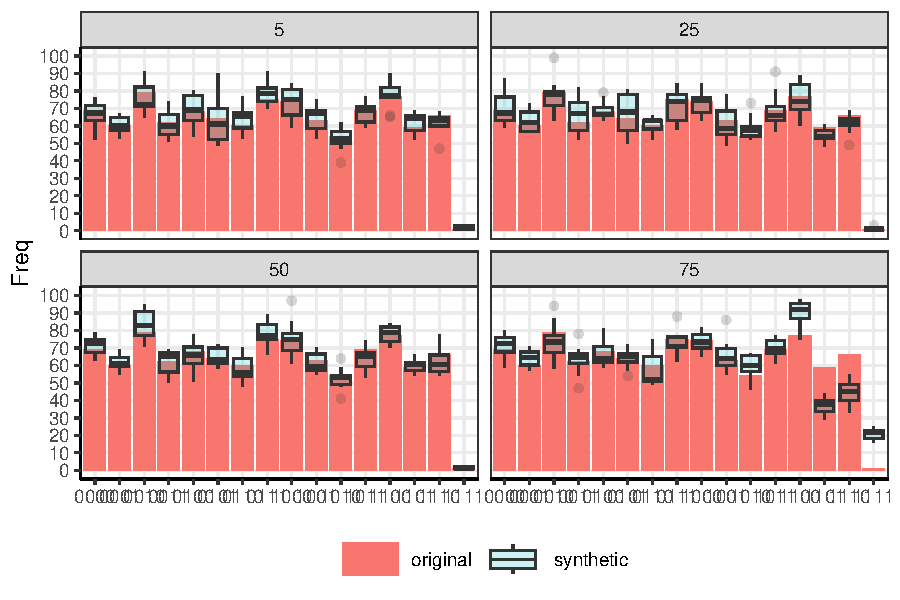
\includegraphics[width=\textwidth]{../../graphs/graph_cart_modified_mb_histogram_compare_10_v2.pdf}
    \end{figure}
\end{minipage}
\hfill
\begin{minipage}{0.48\textwidth}
    \begin{figure}
        \centering
        \caption{cp}
        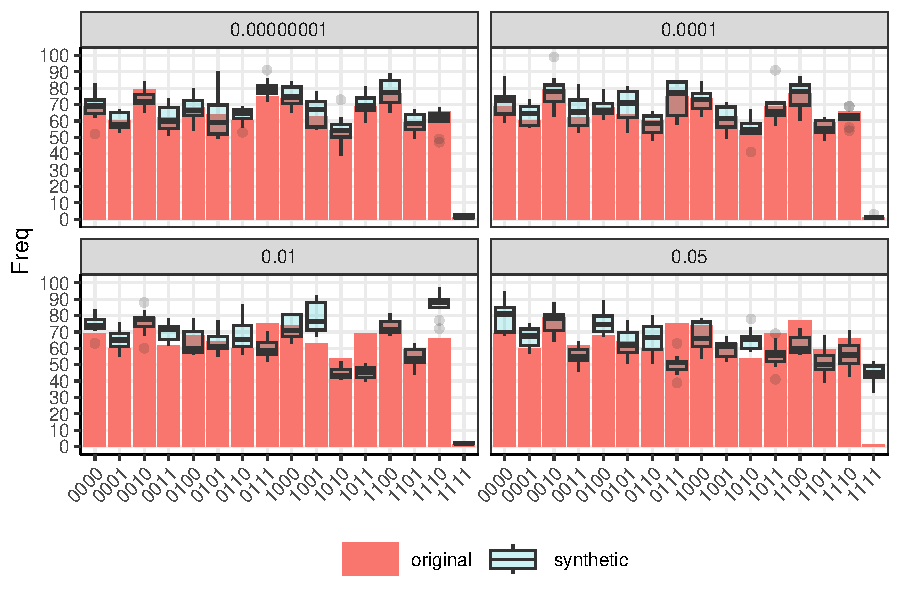
\includegraphics[width=\textwidth]{../../graphs/graph_cart_modified_cp_histogram_compare_10_v2.pdf}
    \end{figure}
\end{minipage}
}

\frame{\frametitle{Illustrating the attack with CART (modified parameters)}
\vskip -4mm
\begin{minipage}{0.48\textwidth}
    \begin{figure}
        \centering
        \caption{mb = 75}
        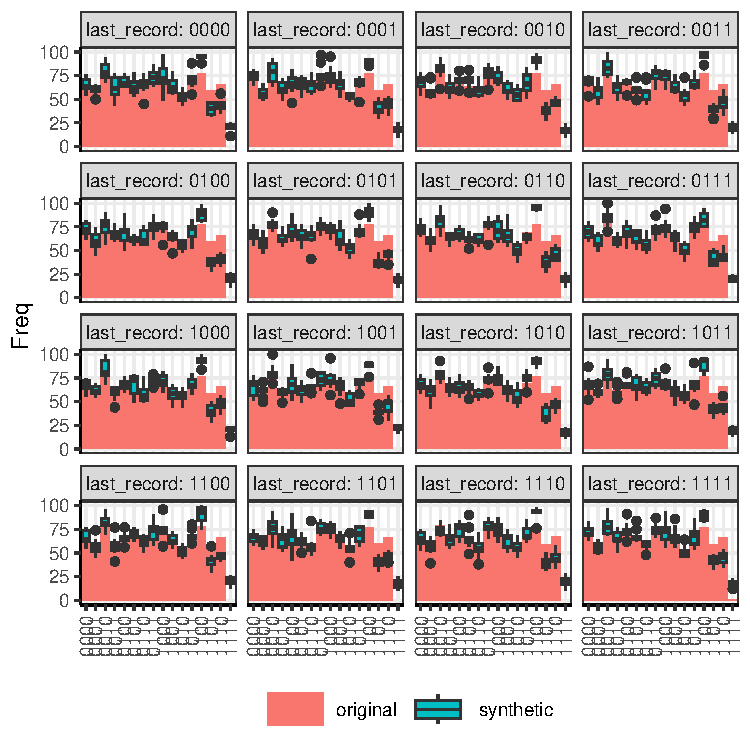
\includegraphics[width=\textwidth]{../../graphs/graph_attacker_modified_mb_v2.pdf}
    \end{figure}
\end{minipage}
\hfill
\begin{minipage}{0.48\textwidth}
    \begin{figure}
        \centering
        \caption{cp = 0.05}
        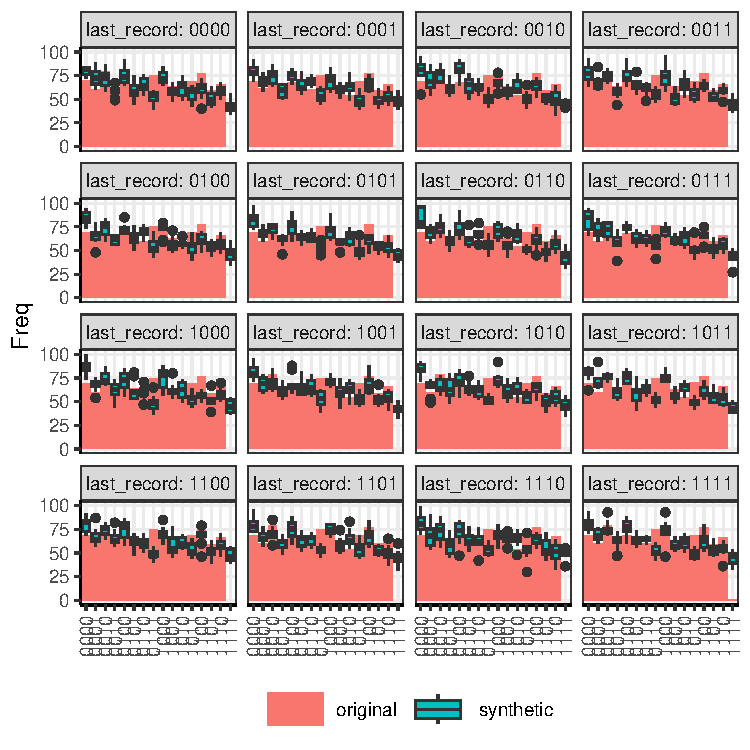
\includegraphics[width=\textwidth]{../../graphs/graph_attacker_modified_cp_v2.pdf}
    \end{figure}
\end{minipage}
}


\frame{\frametitle{Other options: generate noise with $\epsilon$-DP}
\begin{figure}[!h]
    \centering
    \caption{Datasynthesizer with DP}
    \resizebox{\textwidth}{!}{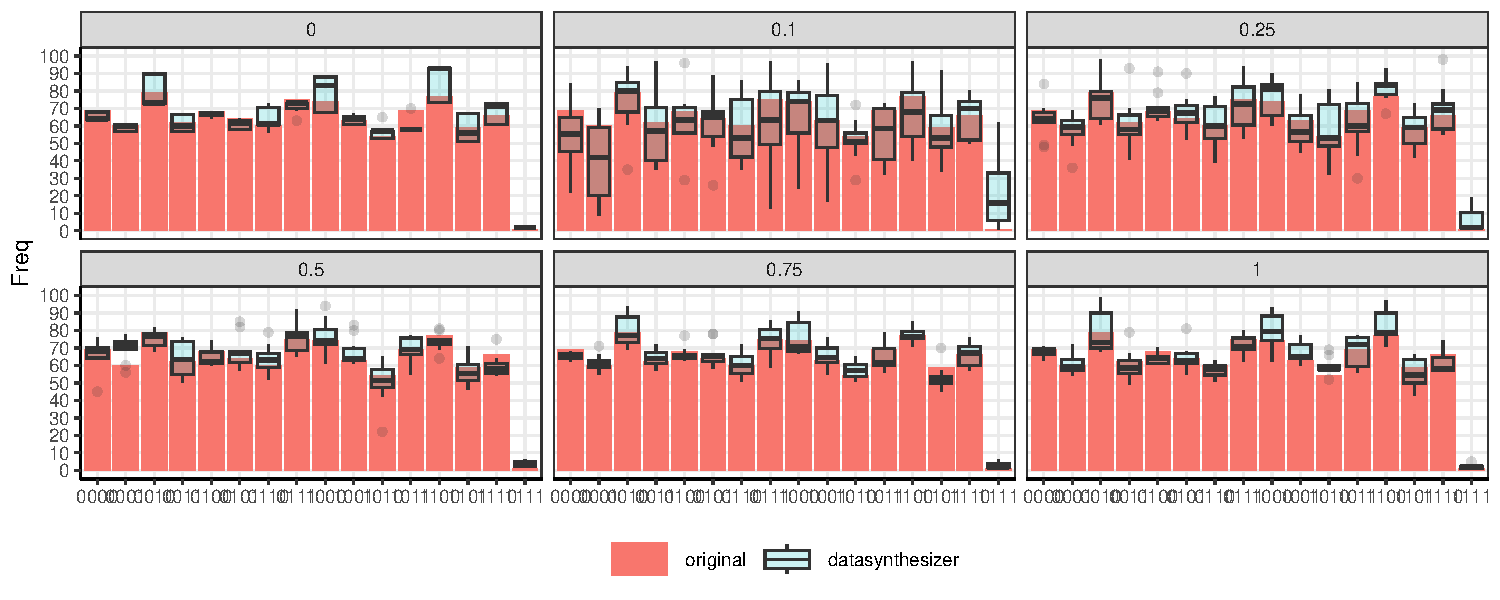
\includegraphics{../../graphs/graph_dp_datasynthesizer_compare_histogram_10_v2.pdf}}
    \label{fig:dp_datasynthesizer}
\end{figure}
}

\frame{\frametitle{Other options: CART (factor) vs. CTREE}
\begin{figure}[!h]
    \centering
    \caption{}
    \resizebox{\textwidth}{!}{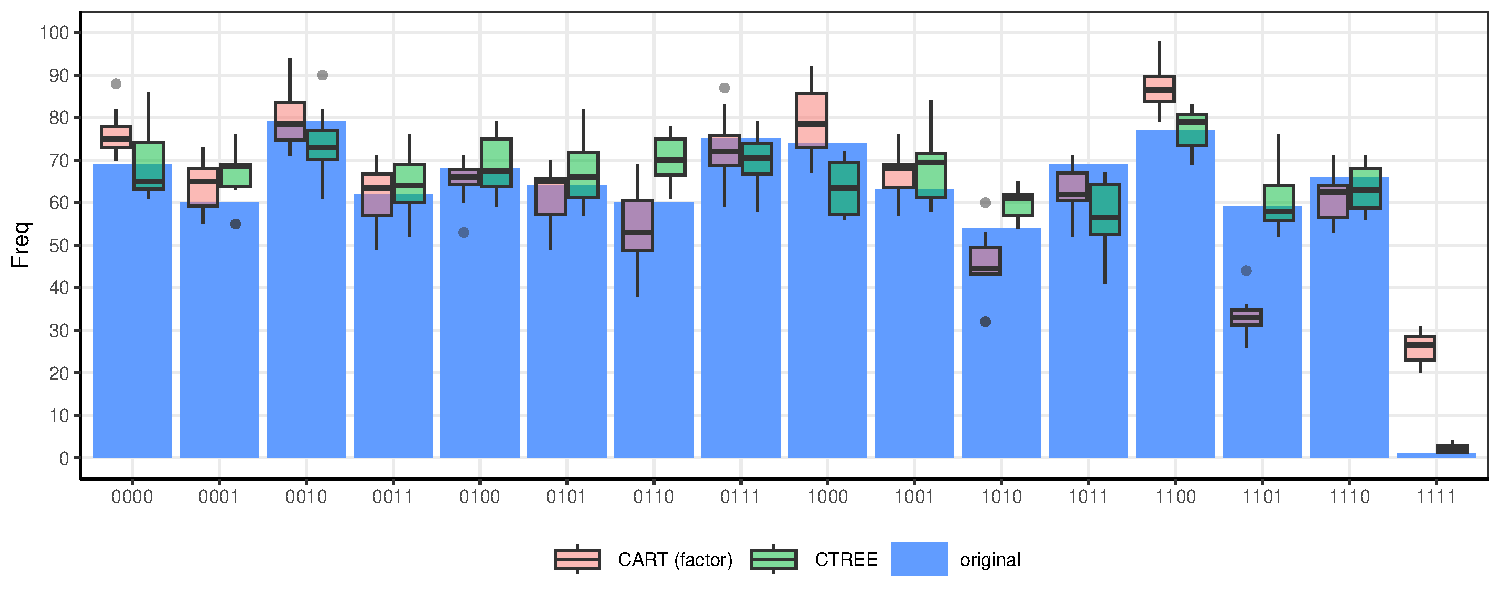
\includegraphics{../../graphs/graph_ctree_cart_factor_histogram_compare_10.pdf}}
    \label{fig:ctree_cart_factor}
\end{figure}
}

\frame{\frametitle{Explaining difference between CART (factor) vs. CTREE}
\begin{figure}[!h]
    \centering
    \caption{}
    \resizebox{\textwidth}{!}{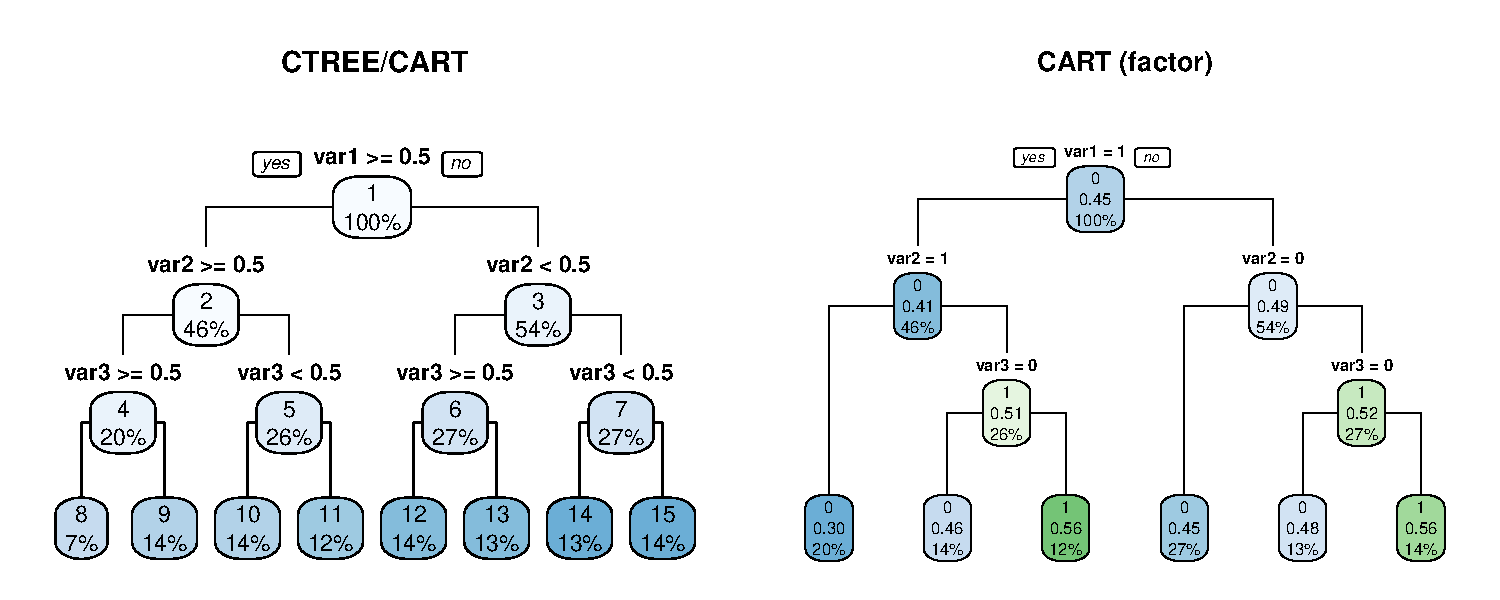
\includegraphics{../../graphs/graph_tree_combined.pdf}}
    \label{fig:tree_combined}
\end{figure}
}

\frame{\frametitle{The bad news}
\begin{itemize}
    \item We don't know how to identify the privacy risk
    \item We have to know a problem exists before we would do something about it
\end{itemize}
}

%%%%%%%%%%%%%%%%%%%%%%%%%%%%%%%%%%%%%%%%
%%%%%%%%%%%%%%%%%%%%%%%%%%%%%%%%%%%%%%%%
\section{Is this scenario realistic?}\label{sec:reality}
%%%%%%%%%%%%%%%%%%%%%%%%%%%%%%%%%%%%%%%%
%%%%%%%%%%%%%%%%%%%%%%%%%%%%%%%%%%%%%%%%
\begin{frame}[c,plain]
\vskip-4mm
\begin{beamercolorbox}[wd=\boxwidth,ht=22.11mm]{transparent}%
    \vfill%
    \usebeamerfont{title}%
    \leftinsert%
    \MakeUppercase{Section \ref{sec:reality}: Is this scenario realistic?
} % <- Hier die Überschrift eintragen
\end{beamercolorbox}
\vskip-3mm
\pgfuseimage{rahmenlinie}

\end{frame}

\frame{\frametitle{Real world data (SD2011)}

Following the authors of Synthpop (Raab, 2024; Raab et al., 2024), we rely on data from Social Diagnosis 2011 (SD2011).  

In their paper, they generate 5 synthetic data sets to illustrate their method for measuring attribute disclosure by identifying values in the target variable \texttt{depress} from keys: \texttt{sex} \texttt{age} \texttt{region} \texttt{placesize}.  

To illustrate why it is a problem to measure attribute disclosure as the set of records with constant $t$ within $q$, we set $t$ as constant for all observations in all 5 synthetic data sets.  0 was chosen because it is the most frequent value in the variable \texttt{depress} (22\% of all records).  By definition, this reduces attribute disclosure risk.  

In their example, attribute risk is about 9\% (as shown in the appendix).  
However, when we modify \texttt{depress}, the risk \emph{increased} to around 15\%.

}


\frame{\frametitle{Results}
\begin{table}[]
    \caption{SD2011}
    \label{tab:attribute_risk_sd2011}
    \centering
    \caption{Attribute disclosure measures for \texttt{depress} from keys: \texttt{sex} \texttt{age} \texttt{region} \texttt{placesize}}
    % \rowcolors{1}{white}{lightgray}
    % latex table generated in R 4.4.0 by xtable 1.8-4 package
% Thu Feb 27 14:39:11 2025
\begin{tabular}{lrrrr}
   
\toprule & 
\multicolumn{2}{l}{Identity risk} &
\multicolumn{2}{l}{Attribute risk}
\\  
 
\cmidrule(lr){2-3}
\cmidrule(lr){4-5}
 
Data & Raab et al., 2024 & Modified & Raab et al., 2024 & Modified
\\ 

\midrule
Original data & 48.38 & 48.38 & 53.30 & 53.30 \\ 
  Synthetic 1 & 14.82 & 14.82 & 8.96 & 14.74 \\ 
  Synthetic 2 & 14.20 & 14.20 & 9.90 & 14.82 \\ 
  Synthetic 3 & 15.16 & 15.16 & 10.46 & 14.94 \\ 
  Synthetic 4 & 14.12 & 14.12 & 9.68 & 14.50 \\ 
  Synthetic 5 & 14.30 & 14.30 & 8.88 & 14.66 \\ 
  Average & 14.52 & 14.52 & 9.58 & 14.73 \\ 
   \bottomrule \\[-1.8ex] \multicolumn{5}{p{4in}}{Note: Modified indicates that values of \texttt{depress}=0  in synthetic data} 
\end{tabular}

\end{table}

}

\frame{\frametitle{Identifying disclosure from 1-way}

The package authors are aware that the $DiSCO$ measure of attribute disclosure risk can indicate a high level of risk for a target variable where a high proportion of records have one level (Raab et al., 2024).

The package includes a flag to allow the user to identify values within a variable that explain most of the disclosures (\texttt{check\_1way}).

The authors give an example where the target variable is \texttt{workab}, where 89\% of the observations never worked abroad.  

The authors suggest that this level of $t$ for a group with the same $q$ would not be disclosive.

We agree, but our example illustrates that the disclosure measure increases, when it should decrease.


}


%%%%%%%%%%%%%%%%%%%%%%%%%%%%%%%%%%%%%%%%
%%%%%%%%%%%%%%%%%%%%%%%%%%%%%%%%%%%%%%%%
\section{Conclusion}\label{sec:conclusion}
%%%%%%%%%%%%%%%%%%%%%%%%%%%%%%%%%%%%%%%%
%%%%%%%%%%%%%%%%%%%%%%%%%%%%%%%%%%%%%%%%
\begin{frame}[c,plain]
\vskip-4mm
\begin{beamercolorbox}[wd=\boxwidth,ht=22.11mm]{transparent}%
    \vfill%
    \usebeamerfont{title}%
    \leftinsert%
    \MakeUppercase{Section \ref{sec:conclusion}: Conclusion} % <- Hier die Überschrift eintragen
\end{beamercolorbox}
\vskip-3mm
\pgfuseimage{rahmenlinie}
\end{frame}

\frame{\frametitle{Summary}
\begin{itemize}
    \item It has long been understood that there is a trade-off between utility and risk
    \item Previous research indicated that CART models were less sensitive to this trade-off than other SDGs 
    \item Using a simulated data set, we show that CART are sensitive to this trade-off
    \item The good news: It is possible to reduce risk in CART with parameters
    \item The bad news:
    \begin{itemize}
        \item Common privacy metrics do not capture risk in our simulated data
        \item We must sacrifice utility
    \end{itemize}
    \item Question: If you did not know there was a problem, why would you sacrifice utility?

\end{itemize}
}

\frame{\frametitle{Thank you}

Jonathan Latner: \url{jonathan.latner@iab.de} \\

Reproducible code: \url{https://github.com/jonlatner/KEM\_GAN/tree/main/latner/projects/simulation} 

}



\end{spacing}
\end{document}

